\documentclass[a4paper]{article}
\usepackage[margin=2.54cm]{geometry}
\usepackage[numbered, framed]{matlab-prettifier}
\usepackage{pdfpages}
\usepackage{parskip}

\lstset{
  style              = Matlab-editor,
  basicstyle         = \mlttfamily,
  escapechar         = ",
  mlshowsectionrules = true,
}


\begin{document}
\section*{Task2}
We trained the network with one hidden layer of 64 neurons, with random initialization of weights.
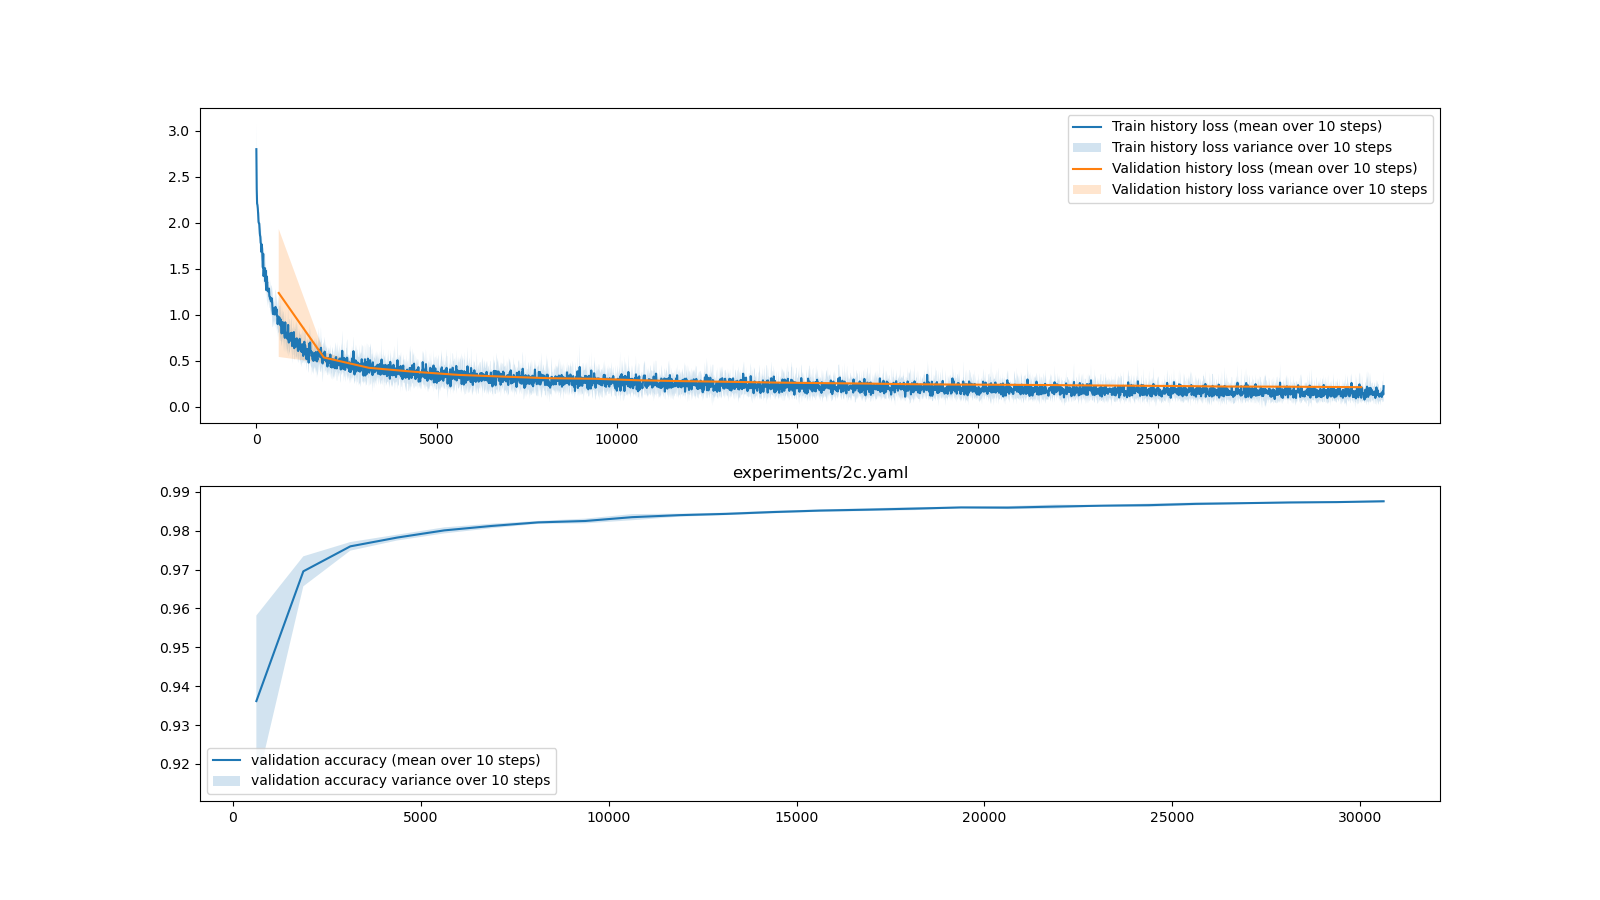
\includegraphics[width=\linewidth]{code/experiments/2c.png}
The network achieves a validation accuracy of $\approx 0.98781 \%$

The network has parameters according to
$$
n_{parameters} = (n_{inputs} + 1) \cdot n_{hidden} + n_{hidden} \cdot n_{out}
$$

Where the term "+1" comes from the bias trick. In our case, this equals

$$
n_{parameters} = (784 + 1) \cdot 64 + 64 \cdot 10 = 50880
$$

Our network has 50880 parameters. This may also be verified through counting the number of elements in the arrays in `model.ws` in the code.

\clearpage
\section*{Task3}
We see that with each trick added, the training improves. Note that early stopping is activated so that 3b and 3c are done much faster than 3a.

\begin{figure}[h]
    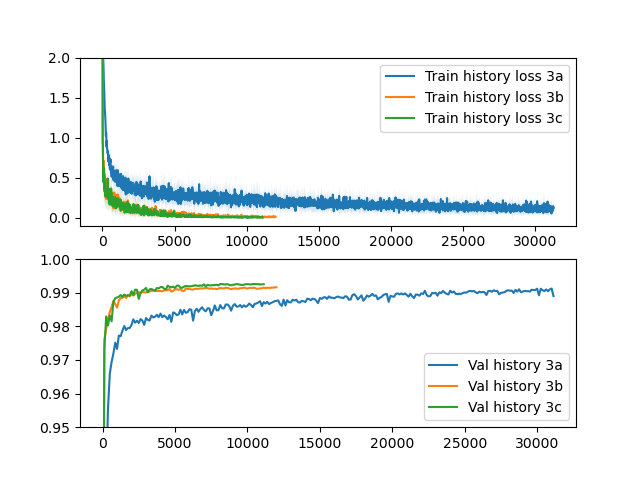
\includegraphics[width=\linewidth]{code/Adding tricks.png}
    \caption{Improvements when adding tricks}
\end{figure}

\clearpage
\section*{Task4}
Comparing the three network structures with different hidden neuron counts: 32, 64 and 128 was interesting.
Clearly having more neurons give a higher accuracy. The biggest difference was computation time - training took slightly longer for the larger nets due to calculating forward and backward are slightly more costly with the bigger matricies.

\begin{figure}[h]
    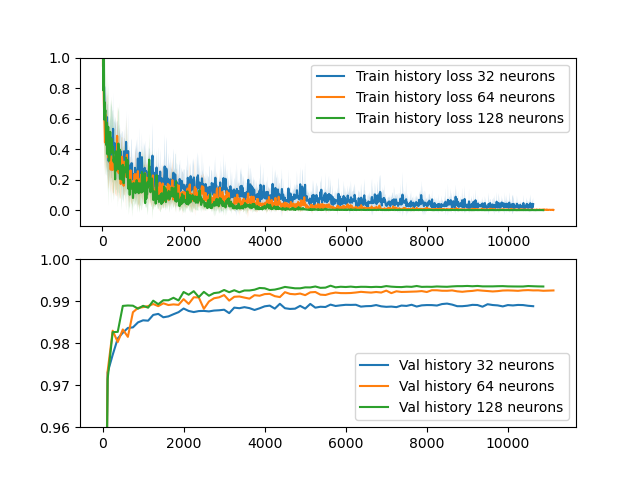
\includegraphics[width=\linewidth]{code/neuron_count_comparison.png}
    \caption{Differences with network structure}
\end{figure}

\clearpage
Comparing two network structures with the same number of parameters, but a different depth was not so interesting.

Using 59 hidden units in both layers, we get approximately the same amount of parameters. In the previous layer we had 50880 parameters, while here we have:
$$
n_{parameters} = (784 + 1) \cdot 59 + 59 \cdot 59 + 59 \cdot 10 = 50386 \approx 50880
$$

They seem to behave very similarly, producing the same accuracy. No difference was observed in training.

This makes sense, as there are basically the same number of parameters to tune. The biggest difference is that the deeper network gets a bit more nonlinearity-opportunity due to the additional layer of sigmoid neurons. This did not have any noticable effect though.

\begin{figure}[h]
    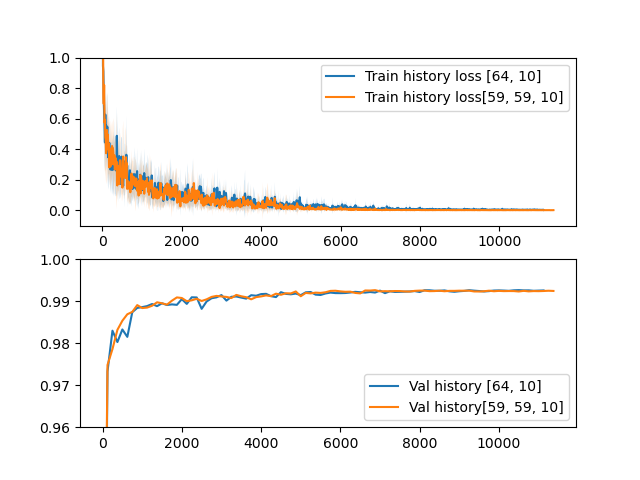
\includegraphics[width=\linewidth]{code/one_vs_two_hidden_layers.png}
    \caption{Differences with one or two hidden layers}
\end{figure}

\clearpage
Training a deep network with 10 hidden layers took some time (numerical from more iterations and more weights), but it did not yield any big differenes in performance. The two nets are very similar.

\begin{figure}[h]
    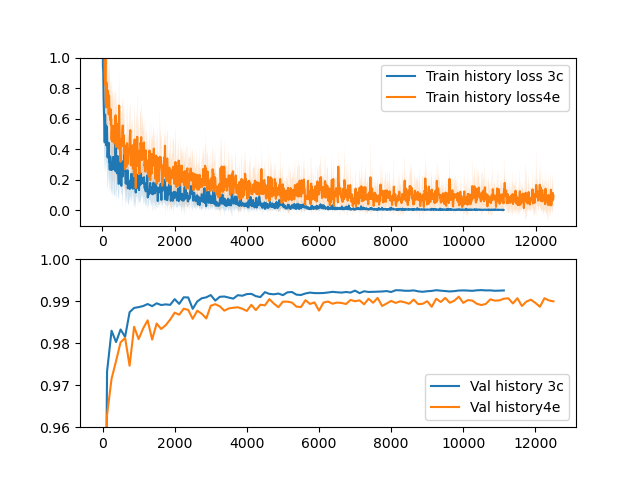
\includegraphics[width=\linewidth]{code/deeeeep_network.png}
    \caption{Differences with deep vs shallow network}
\end{figure}


\end{document}